\documentclass[12pt]{article}

\usepackage{amssymb, amsthm, linguex, enumerate, amsmath}

% Language setting
% Replace `english' with e.g. `spanish' to change the document language
\usepackage[english]{babel}

% Set page size and margins
% Replace `letterpaper' with`a4paper' for UK/EU standard size
\usepackage[letterpaper,top=2cm,bottom=2cm,left=3cm,right=3cm,marginparwidth=1.75cm]{geometry}

% Useful packages
\usepackage{amsmath}
\usepackage{graphicx}
\usepackage{enumitem}
\usepackage{xcolor}
\usepackage[colorlinks=true, allcolors=blue]{hyperref}

\newcommand{\R}{\mathbb{R}}
\newcommand{\x}{x \in \mathbb{R}}
\newcommand{\nat}{n \in \mathbb{N}}
\newcommand{\dx}{\frac{d}{dx}}
\newcommand{\dxof}[1]{\frac{d}{dx} \left( {#1} \right) }
\newcommand{\E}[1]{E\left( {#1} \right)}
\newcommand{\pars}[1]{\left( {#1} \right) }
\newcommand{\brac}[1]{\left[ {#1} \right] }
\newcommand{\limit}[3]{\lim_{{#1}\to {#2}} {#3}}
\newcommand{\xo}{x_0}
\newcommand{\iid}{independent identically distributed }
\newcommand{\dble}{differentiable }
\newcommand{\xbar}{\bar{X}}
\newcommand{\ybar}{\bar{Y}}
\newcommand{\rv}{random variable }
\newcommand{\distn}{distribution }
\newcommand{\cont}{continuous }
\newcommand{\disc}{discontinuous }
\newcommand{\forx}{\qquad \text{for all } x}
\newcommand{\cbi}{closed bounded interval }
\newcommand{\seq}[1]{\{{#1}\}}
\newcommand{\limn}{\lim_{n\to\infty}}
\renewcommand{\f}[1]{f^{({#1})}}
\renewcommand{\sup}[1]{\text{sup}\left\{ {#1} \right\}}
\renewcommand{\inf}[1]{\text{inf}\left\{ {#1} \right\}}
\newcommand{\N}[2]{N \left( {#1},{#2} \right)}
\newcommand{\gammaDist}[2]{\gamma \left( {#1},{#2} \right)}
\newcommand{\Ndef}{N\left(\mu, \sigma^2\right)} %default normal
\newcommand{\thru}[1]{{#1}_1, \dots, {#1}_n}
\newcommand{\yn}{Y_1, \dots, Y_n}
\renewcommand{\max}[1]{\text{max}\left\{ {#1} \right\}}
\renewcommand{\min}[1]{\text{min}\left\{ {#1} \right\}}
\renewcommand{\over}[1]{\frac{1}{{#1}}}
\renewcommand{\P}[1]{P \left( {#1} \right) }
\newcommand{\prob}[1]{P \left( {#1} \right) }
\newcommand{\nl}{\vspace{0.1in}\noindent}
\newcommand{\nnl}{\vspace{0.2in}\noindent}
\title{Math 326 - Probability $\&$ Statistics II}
\author{Matt Wilder}

\begin{document}
\maketitle

\section*{MTH 326 Notes}
\section*{1/19/2022 Day 1}
\section*{Chapter 7 - Review}
Our first goal in Math 326 is to learn how to estimate global parameters of "population" like $\mu$ and $\sigma$. To do this, we need to understand how the random variable we use to estimate these are distributed.
$$\left\{\begin{aligned}
    \mu & \qquad \bar{X} = \over{n} \sum X_i
    \\
    \sigma^2 & \qquad S^2 = \over{n-1} \sum \pars{X_i - \xbar}^2
    \end{aligned}\right.$$

%/text{"<piecewise>" eg, $\mu \qquad , \bar x = 1/n \sum x_i \n sigma^2 \qquad , s^2 = 1/(n-1) sum (x_i - xbar)^2$}

\section*{$\S$ 7.2 - Sample Means}
\textbf{Theorem 7.1}: Let $\yn$ be a random sample from $\Ndef$ then $\ybar$ is distributed by $\N{\mu}{\frac{\sigma^2}{n}}$. The distribution of sample means, $\ybar$, is also Normal.
\\\\Reason: Linearity of Expectation and Variance properties
\\\\\emph{Recall:}
\begin{enumerate} %[label=\textbf{\roman*}.]
        \item In working with $\Ndef$, we learned it was easier to standardize everything via
        $Z$-scores. $$Z = \frac{x-\mu}{\sigma}$$
        and $Z$ is distributed $\N{0}{1}$, the \textbf{Standard Normal Distribution.}
        
        \item Sample variance. Recall standard deviation $\sigma$ is a measure of spread of the variable and its derived from $\pars{Y_i - \ybar}^2$ terms.
 In all math, we normalize to take the "units" out of things.
 $$U_i = \frac{Y_i - \bar{Y}}{S} \approx \frac{Y_i - \mu}{\sigma} = Z_i$$
    \end{enumerate}
Data driven ($\frac{Y_i - \bar{Y}}{S}$), it is a statistic. However, ($\frac{Y_i - \mu}{\sigma}$) is not a statistic.
Reason: It is derived on unknown population parameters, none-the-less, it makes it easier to predict and start from here.
\\\\\textbf{Theorem 7.2} If $\yn$ are a random sample of $\Ndef$, then
$$U = \sum Z_i^2 = \sum \pars{\frac{Y_i - \mu}{\sigma}}^2$$
has a $\chi ^2$ distribution with $n$ degrees of freedom.
\\\\\textit{Recall}: $\chi^2$ distribution is a $\gammaDist{\frac{v}{2}}{2}$ where $v = $ degrees of freedom.
\\\\Reason: All this $Z_i^2$ is $\chi^2$ with df=1, 
By products of mgf (moment generating function), $\sum Z_i^2$ is $\chi^2$ with $n$ degrees of freedom.
Now to get sample variance, we algebra:
\begin{align}
        S^2 &= \frac{1}{n-1}\sum(Y_i-\bar{Y})^2 \notag\\
        & \approx \frac{1}{n-1}\sum(Y_i - \mu)^2 \notag
    \end{align}
$$\frac{S^2}{\sigma^2} \approx \frac{1}{n-1}\sum \pars{\frac{Y_i - \mu}{\sigma}}^2$$
$$\frac{S^2\cdot(n-1)}{\sigma^2} \approx \sum Z_i^2$$
Showing it is okay to replace $\ybar$ with $\mu$ is the point of the proof of...
\\\\\textbf{Theorem 7.3 (Fisher's Theorem)} The distribution of sample variance $S^2$
\\If $\yn$ is a random sample from $\Ndef$ then 
\begin{enumerate}
        \item $\frac{S^2\cdot(n-1)}{\sigma^2}$ has $\chi^2$ distribution with $(n-1)$ degrees of freedom
        \item  $\bar{Y}$ and $S^2$ are independent random variables
        \item $t$-distribution and $f$-distribution
$$\frac{Y_i-\mu}{\sigma} \approx \frac{Y_i -\mu}{S} \approx \frac{Y_i - \bar{Y}}{S}$$
$$\text{Normal} \approx \text{t-dist'n} \approx \text{stat}$$
    \end{enumerate}
Address when to use what is the point of this class
\\Skip definitions (such as moments) for the time being
\\Also, The Law of Large Numbers. Used to prove the CLT (Central Limit Theorem)
\section*{$\S$ Section 7.4 - The Central Limit Theorem}
The reason Normal distributions play an outsized role in applies stats is that the distribution of of $\bar{Y}$ can be made \emph{nearly normal}, no matter the underlying distribution of $Y$ (Does not need to start 'life' Normal)
So nearly normal, we just pretend that it is.
\\\\\textbf{Theorem: The Central Limit Theorem}\\
Let $\yn$ be independent and identically distribution (iid) random variable with
$$E\pars{Y_i} = \mu \qquad \text{and} \qquad V(Y_i) = \sigma^2 < \infty$$
(Need finite variance for CLT to hold)\\
Define $$U_n = \frac{\bar{Y}-\mu}{\sqrt{\frac{\sigma^2}{n}}} = \frac{\sum (Y_i) - n\mu}{\sigma \sqrt{n}}$$
The CLT says the distribution function of $U_n \to N(0,1)$ as $n\to\infty$
\\Big idea: The distribution $\ybar$ can be thought of as $\N{\mu}{\frac{\sigma^2}{n}}$.
\\\\\textbf{Example:} Let $\xbar$ denote the mean of a random sample of size $n=15$, from the distribution whose pdf is $$f(x) = \frac{3}{2}x^2, \qquad x \,\in\, [-1,1]$$
\textit{Aside:} \textbf{Support}: the domain on which $f$ is non-zero. \\
Can be shown $$\mu = E[X] = 0 \qquad \text{and} \qquad \sigma^2 = E((X-\mu)^2) = \frac{3}{5}$$
To compute $P\pars{0.03 \leq \bar{X} \leq 0.15}$ use the CLT and assume $\bar{X}$ is distributed $\N{0}{\frac{3/5}{15}} = \N{0}{1/25}$.
Then
\begin{align}
        P\pars{0.03 \leq \bar{X} \leq 0.15} &= P\pars{\frac{0.03-\mu}{\sqrt{1/25}} \leq \frac{\xbar - \mu}{\sigma} \leq \frac{0.15-\mu}{\sqrt{1/25}}} \notag\\
        &= P\pars{\frac{0.03-\mu}{\sqrt{1/25}} \leq Z \leq \frac{0.15-\mu}{\sqrt{1/25}}} \notag\\
        &=  P\pars{\frac{0.03-0}{\sqrt{1/25}} \leq Z \leq \frac{0.15-0}{\sqrt{1/25}}} \notag \\
        & =  P\pars{\frac{0.03}{\sqrt{1/25}} \leq Z \leq \frac{0.15}{\sqrt{1/25}}} \notag\\
        &= P\pars{0.15\leq Z \leq 0.75} \notag \\
        &= \text{Table4}(0.15) - \text{Table4}(0.75)\notag\\
        &= 0.7734 - 0.5596 \notag\\
        &= 0.2138 \notag
    \end{align}
Recall that Table 4 gives upper tail probabilities.
\newpage
\section*{1/21/2022 Day 2}
\section*{Chapter 8: Estimation}
\section*{$\S$ 8.1 An Estimator}
We are seeking an unknown population parameter. General name, $\theta$, (e.g. $\mu$, $\sigma^2$, $\rho$, ...).\\
The rule used to approximate or guess $\theta$ is called an \textbf{\underline{estimator}}. Any guess, based on observations is an \textbf{\underline{estimate}}.\\
\\\textbf{e.g.}\\

What $\theta = \mu$\\
Estimator:
$$\underbrace{\xbar = \over{n} \sum x_i}_{\text{a function}}$$
If we had 7 observations, $Y_1, \dots, Y_7$, then
$\ybar = \over{7} \sum_1^7 Y_i$ is an \underline{estimate}.\\
These are also \textbf{\underline{interval estimators}}.
\\\\\textbf{e.g. }\\

Confidence interval, $\theta = \mu$
$$\xbar - SZ_x \leq \mu \leq \xbar + SZ_x \qquad\qquad |\xbar - \mu | \leq SZ_x$$
\vspace{0.3in}
\section*{$\S$ 8.2}
A start at trying to determine if an estimator is any good.\vspace{0.08in}\\
Let $\hat{\theta}$ be a point estimator for a parameter $\theta$. (e.g. $\theta = \mu, \quad \hat{\theta} = \xbar$)
\begin{enumerate}[label=\textbf{\arabic*}.)]
    \item One goal of a good estimator is that $\E{\hat{\theta}} = \theta$\\\\\textbf{e.g.} by CLT, $E[\xbar] = \mu$\\\\
But this is not always the case.\\
\\\textbf{Def:} If $E[\hat{\theta}]=\theta$, we say that $\hat{\theta}$ is an \textbf{\underline{unbiased}} estimator. (e.g. $\xbar$ is unbiased).\\
If $\hat{\theta}$ is a biased point estimator, we define the bias to be
$$B(\hat{\theta}) = E(\hat{\theta}) - \theta$$
    \item  Another goal of a good estimator might be that its "spread" is tightly packed (hopefully about $\theta$)
$$\text{spread}\, \Longrightarrow \text{variance}$$
\textbf{Def:} The \textbf{\underline{mean square error}} of $\hat{\theta}$ is
$$MSE(\hat{\theta}) = E\brac{(\hat{\theta} - \theta)^2}$$
Recall: $V[X] = E[X^2] - (E[X])^2$\\
Corollary:
$$MSE(\hat{\theta}) = V(\hat{\theta}) + [B(\hat{\theta})]^2$$
\begin{proof}
    \begin{align}
        MSE(\hat{\theta}) &= E(\hat{\theta}^2 - 2\hat{\theta}\cdot \theta + \theta ^2) \notag\\
        &= E[\hat{\theta}^2] - 2E(\hat{\theta}\theta) +E(\theta ^2) \notag\\
        &= E(\hat{\theta}^2) - 2E(\hat{\theta})\theta + \theta^2 \notag \\
        &= E(\hat{\theta}^2) - (E(\hat{\theta}))^2 + (E(\hat{\theta}))^2 - 2E(\hat{\theta})\theta + \theta ^2\notag\\
        &= V(\hat{\theta}) + (E(\hat{\theta})-\theta)^2\notag\\
        &= V(\hat{\theta}) + (B(\Hat{\theta}))^2\notag
    \end{align}
\end{proof}
\textit{Remark:} We have decomposed MSE
$$MSE(\hat{\theta}) = \underbrace{V(\hat{\theta})}_{\text{Precision}} + \underbrace{B(\hat{\theta})^2}_{\text{Accuracy}}$$
\end{enumerate}
Idea of a "best" estimator is tricky. We'd like MSE to be as small as possible, but usually is an impossible problem because MSE depends on the unknown $\hat{\theta}$.\\\\
\textbf{ex:} (Population proportions).\\\\

Want $p$. Let
$$Y = \begin{cases} 
      1 & \text{success} \\
      0 & \text{failure} 
   \end{cases}$$
$\{Y_i\}$ a iid random sample.\\
\\Estimator 1: $\hat{p} = \over{n}\sum Y_i = \ybar$, sums the $\frac{\text{people said yes}}{\text{total}}$\\\\
Recall that $\sum Y_i$ is $\text{binom}(n,p)$.\vspace{0.35in}\\
And for a Binomial Distribution, we know
$$E[X] = np \qquad \text{and} \qquad V[X] = npq = np(1-p)$$
Then what is the $E[\hat{p}]$?
$$E[\hat{p}] = E\pars{\over{n}\sum Y_i} = \over{n}E\pars{\sum Y_i} = \over{n}\cdot np = p$$
Therefore $\hat{p}$ is an unbiased estimator.
$$V(\hat{p}) = V\pars{\over{n}\sum Y_i} = \pars{\over{n}}^2V\pars{E\sum Y_i} = \pars{\over{n}}^2 np(1-p) = \frac{p(1-p)}{n}$$
and $$\text{MSE}(\hat{p}) = \frac{p(1-p)}{n} + \underbrace{0^2}_{\text{"unbiased"}}$$
\\\textbf{Estimator 2}: 
$$\Tilde{p} = \frac{\sum_1^n Y_i + 1}{n+2}$$
note:
$$n = 1, \qquad y = \begin{cases} 
      1\\
      0
   \end{cases} \qquad \tilde{p} = \begin{cases} 
      2/3 & \\
      1/3 \\
   \end{cases}$$
   $$n = 2, \qquad y = \begin{cases} 
      2\\
      1\\
      0
   \end{cases} \qquad \tilde{p} = \begin{cases} 
      3/4 \\
      2/4\\
      1/4
   \end{cases}$$
$$E[\Tilde{p}] = \over{n+2}\pars{E\pars{Y_i} + E(1)} = \frac{np+1}{n+2} = p + \frac{1-2p}{n+2} = p$$
So $\tilde{p}$ is biased
$$B(\tilde{p}) = E(\tilde{p}) - p = p + \frac{1-2p}{n+2} - p = \frac{1-2p}{n+2}$$
Calc question:

What happens to $E[\tilde{p}]$ as sample size grows? ($E\pars{\tilde{p}} \to p$)\\\\
Need
\begin{align}
    V(\tilde{p}) &= V\pars{\frac{\sum_1^n y_i + 1}{n+2}} \notag\\&=  V\pars{\frac{\sum_1^n y_i}{n+2} + \over{n+2}} \notag\\&= V\pars{\frac{\sum_1^n y_i}{n+2}} \notag\\ &= \over{(n+2)^2} V\pars{\sum Y_i} \notag\\ &= \frac{np(1-p)}{(n+2)^2}\notag
\end{align}
Then
$$\text{MSE}(\tilde{p}) = \frac{np(1-p)}{(n+2)^2} + \pars{\frac{1-2p}{n+2}}^2 = \frac{np(1-p) + (1-2p)^2}{(n+2)^2}$$
\\\textbf{Q:} Which estimator is better? \hspace{0.25in} \textbf{A:} \textit{it depends!}\\\\
Note MSE a function of \underline{both} $n$ and $p$
$$n = 10, \qquad p \in[0,1]$$
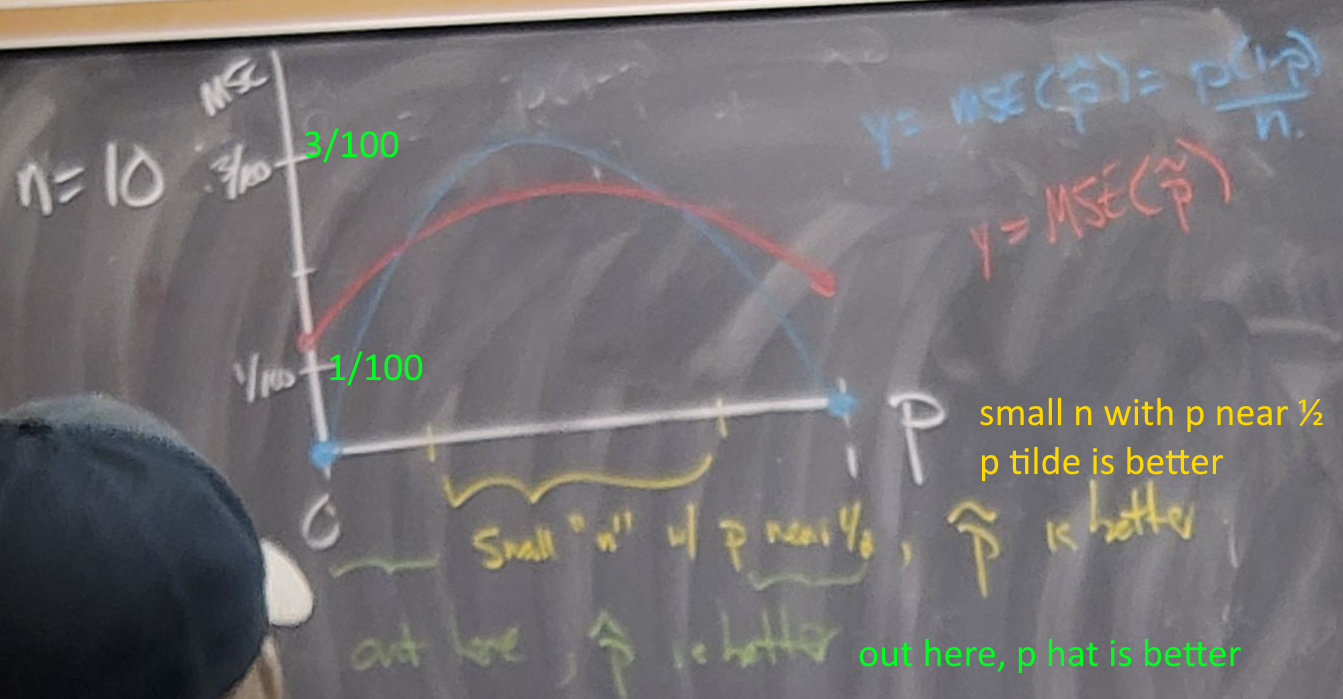
\includegraphics[width=15cm]{mse n 10.png}
\\$$n = 25 \text{ and } 100 \qquad p \in [0,1]$$
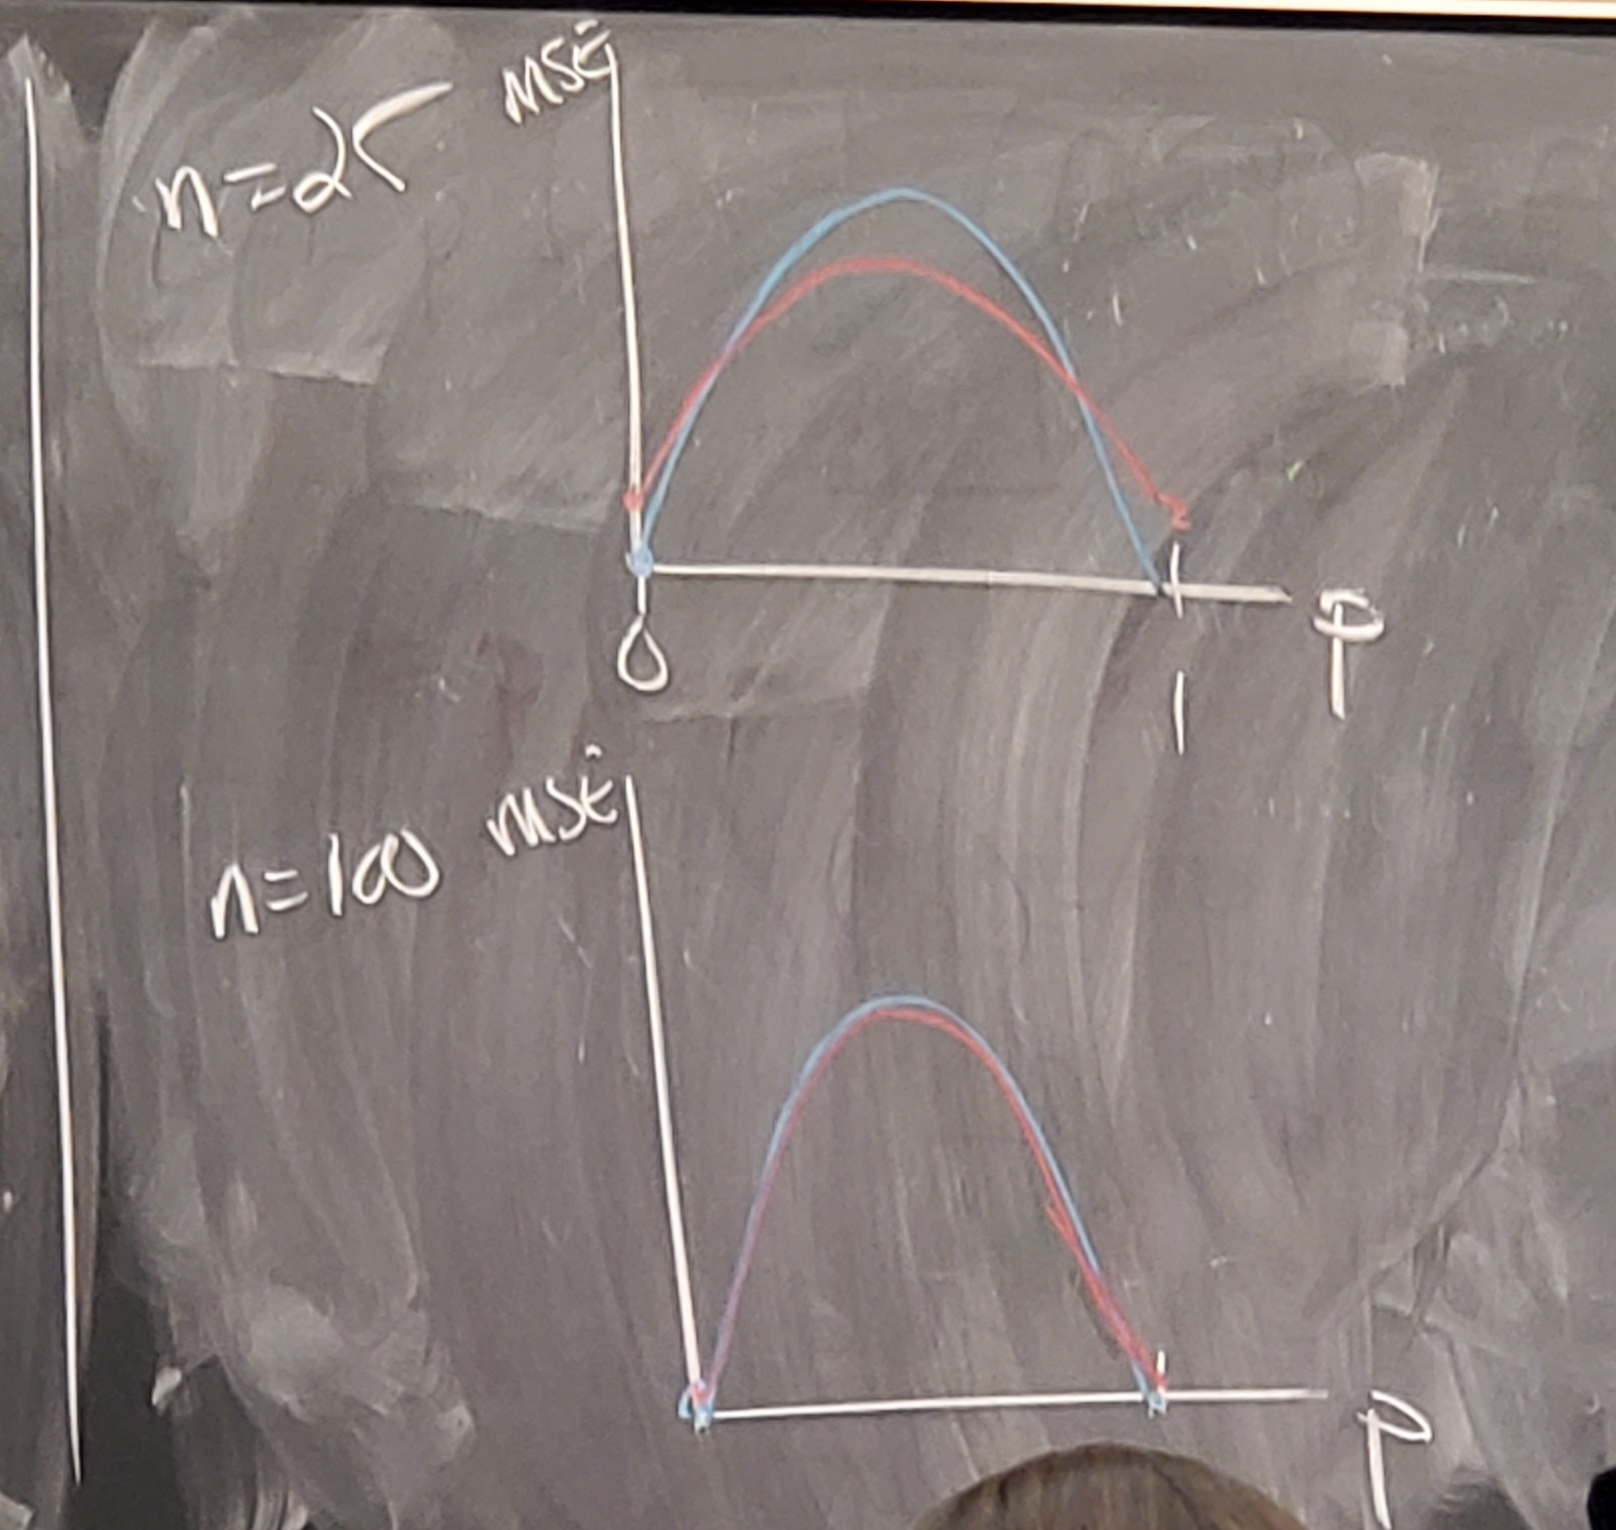
\includegraphics[width=9cm]{mse 25 and 100.png}
%
%
%
%
\newpage
\section*{1/24/2022 Day 3}
\section*{$\S$ 8.3}
Table 8.1, pg 397, Common unbiased estimator for $\mu$, $\rho$, $\mu_1 - \mu_0$, $\rho_1 - \rho_0$.
\vspace{0.25in}\\
\textbf{e.x.} Variance of a data set and the $n-1$.\\\\
Natural definition is $S^2 = \over{n} \sum \pars{X_i-\xbar}^2$\\\\
Why do we use $n-1$?\\
Check $B(S^2)$. Is $E[S^2] = \sigma^2$?\\\\
$$\text{Let} \quad E(X) = \mu \qquad \text{and}\qquad V(X) = \sigma^2$$
and $X_1, \dots, X_n$ iid random sample. Then
\begin{align}
    E(S^2) &= E\brac{\over{n}\sum \pars{X_i - \xbar}^2} \notag\\
    &= \over{n}\underbrace{E\brac{\sum \pars{X_i^2 - 2x_i\xbar + \xbar ^2}}}_{\text{focus on this}}\notag\\
    &= \over{n}\pars{E\brac{\sum X_i^2 - 2\sum X_i\xbar + \sum \xbar^2}}\notag\\
    &= \over{n}\pars{\underbrace{E\brac{\sum X_i^2}}_1 - \underbrace{2E\brac{\sum X_i\xbar}}_2 + \underbrace{E\brac{\sum \xbar}^2}_3} \notag
\end{align}
    1 and 3 uses the "trick" $V(Y) = E(Y^2) - (E(Y))^2$, so
\begin{align}
    \text{Part 1 } &= E\brac{\sum X_i^2} \notag\\ 
    &= \sum E\brac{X_i^2}\notag\\
    &= \sum_1^n \pars{V\brac{X_i} + \pars{E\brac{X_i}}^2}\notag\\
    &= \sum_1^n \pars{\sigma^2 + \mu^2} \notag\\
    &= n\pars{\sigma^2 + \mu^2}\notag
\end{align}
\begin{align}
    \text{Part 3 } &= E\brac{\sum \xbar^2} \notag\\
    &= \sum \pars{V\brac{\xbar} + \pars{E\brac{\xbar}}^2}\notag\\
    &= \sum \pars{\frac{\sigma^2}{n} + \mu^2}\notag\\ %since xbar dist by N(mu, sig^2/n)
    &= n \pars{\frac{\sigma^2}{n} + \mu^2} \notag\\
    &= \sigma^2 + n \mu^2\notag
\end{align}
\begin{align}
    \text{Part 2 } &= -2E\brac{\sum_i X_i\pars{\over{n}\sum_j X_j}}\notag\\
    &= -\frac{2}{n} E \brac{\sum_i \sum_j X_i X_j} \notag\\%n^2 terms
    &= -\frac{2}{n} E \brac{\underbrace{\sum_i X_iX_j}_{n \text{ terms}} + \underbrace{\mathop{\sum\sum}_{i\neq j}  X_i X_j}_{n^2-n \text{ terms}}} \notag\\
    &= -\frac{2}{n} \pars{\underbrace{\sum_i E\brac{X_i^2}}_{\text{this is part 1 again}} + \underbrace{ \mathop{\sum\sum}_{i\neq j}  E\brac{X_i X_j}}_{\text{covariance like}}}\notag
\end{align}
Recall that
\begin{align}
    Cov(X_i,X_j) &= \E{\pars{X_i - \xbar}\pars{X_j - \xbar}} \notag\\
    &= \E{X_iX_j} - \E{X_i}\E{X_j} \notag
\end{align}
But iid, "i" for independent, $\Rightarrow Cov(X_i, X_j) = 0$
$$\therefore \E{X_i X_j} = \E{X_i}\E{X_j} = \mu \cdot \mu = \mu^2$$
\begin{align}
    \text{Part 2 } &= -\frac{2}{n}\Big(n(\sigma^2 + \mu^2) + (n^2 - n)\mu^2\Big)\notag\\
    &= -2\brac{(\sigma^2-\mu^2) + (n-1)\mu^2}\notag
\end{align}
Substituting back into the original parts,
\begin{align}
    E(S^2) &= \over{n}\pars{\underbrace{E\brac{\sum X_i^2}}_1 - \underbrace{2E\brac{\sum X_i\xbar}}_2 + \underbrace{E\brac{\sum \xbar}^2}_3} \notag\\
    &= \over{n}\pars{\underbrace{n(\sigma^2+\mu^2)}_1 - \underbrace{2\Big( \pars{\sigma^2 + \mu^2} + (n-1)\mu^2 \Big) }_2 + \underbrace{\sigma^2 + n\mu^2}_3} \notag\\
    &= \over{n}\pars{\underbrace{n\sigma^2+n\mu^2}_1 \underbrace{ -2\sigma^2 -2\mu^2 -2(n-1)\mu^2}_2 + \underbrace{\sigma^2 + n\mu^2}_3} \notag\\
    &= \over{n}\pars{\underbrace{n\sigma^2\color{red}{+n\mu^2}}_1 \underbrace{ -2\sigma^2 \color{blue} -2\mu^2 \color{red}{-2n\mu^2} \color{blue} + 2\mu^2}_2 + \underbrace{\sigma^2 \color{red}{+n\mu^2}}_3} \notag\\
    &= \over{n}\pars{n\sigma^2 -2\sigma^2 + \sigma^2} \notag\\
    &= \over{n}\pars{n\sigma^2 -\sigma^2} \notag\\
    &= \frac{\sigma^2(n-1)}{n} \notag\\
    &\neq \sigma^2\notag 
\end{align}
Therefore, it is a biased point estimate.\\
To make an unbiased estimator, rescale the natural definition...
$$S = \over{n-1} \sum_1^n \pars{X_i - \xbar}^2$$
\vspace{0.3in}
\section*{$\S$ 8.4 Probability Statements About $\hat{\theta}$}
Definition: Given any $\hat{\theta}$ the exact (theoretical) error is defined as
$$\varepsilon = \left| \hat{\theta} - \theta \right|$$
Note that $\varepsilon$ is itself a r.v. and thus we can make probability statements about it.
\vspace{0.2in}\\Obviously want $\varepsilon$ small.
\vspace{0.1in}\\Consider $\left| \hat{\theta} - \theta \right| < b$
\\We can make conclusions about
$$P\pars{\left| \hat{\theta} - \theta \right| < b}$$
\vspace{0.15in}\\
Chebyshev: $$P\pars{\left| \hat{\theta} - \theta \right| < k\sigma} > 1 - \over{k^2}$$
Remark: We call $\sigma = \sqrt{\sigma^2}$ the \underline{standard error} in stats.\vspace{0.1in}\\
In practice, $k = 2$ is a common choice.
$$P\pars{\left| \hat{\theta} - \theta \right| < 2\sigma} > 1 - \over{2^2} = \frac{3}{4}$$
In real world, $2\sigma$ is usually much better than this (see table 8.2). when the underlying distribution
$\hat{\theta}$ is symmetric and unimodal. \\
Last working assumption for a few lectures: in real life we use $S^2 \approx \sigma^2$\\\\
\textbf{e.g.} (Difference in means)\\

2 iid random samples:
$$n_1 = 100 \qquad \bar{Y_1} = 26400 \qquad S_1^2 = 1440000$$
$$n_2 = 200 \qquad \bar{Y_2} = 25100 \qquad S_2^2 = 1960000$$\vspace{0.05in}\\
Estimating difference in means $\mu_1 - \mu_2$. Here,
$$\bar{Y_1} - \bar{Y_2} = \underbrace{26400 - 25100}_{\text{a point estimate}} = 1300$$
Use $S^2_{\bar{Y_1} - \bar{Y_2}}$ to find a $2\sigma$ interval estimate
$$\sigma^2_{\bar{Y_1} - \bar{Y_2}} \approx S^2_{\bar{Y_1} - \bar{Y_2}} = \frac{S_1^2}{n_1} + \frac{S_2^2}{n_2} \approx \frac{1440000}{100} + \frac{1960000}{200} = 22800$$
$$\sigma_{\bar{Y_1} - \bar{Y_2}} \approx S_{\bar{Y_1} - \bar{Y_2}} = \sqrt{S_{\bar{Y_1} - \bar{Y_2}}^2} = \sqrt{22800} \approx 151$$
\\a $2\sigma$ interval estimate for $\mu_1 - \mu_2$ is $1300 \pm 2(151) \Rightarrow 1300 \pm 302 \text{ or } (998, 1602)$
\vspace{0.3in}
\section*{$\S$ 8.5 Confidence Intervals}
Goal: Take interval estimates for $\S$8.4 but make more precise comments about the probability $P\pars{\left| \hat{\theta} - \theta \right| < k\sigma}$
$$-k\sigma < \hat{\theta}-\theta < k\sigma \longrightarrow \hat{\theta} - k \sigma < \theta < \hat{\theta} + k\sigma$$
consider
$$P\pars{\hat{\theta}_L \leq \theta \leq \hat{\theta}_u} = 1 - \alpha$$
$\hat{\theta}_L$, $\hat{\theta}_U$ lower and upper \underline{confidence limit.}
\\$1-\alpha$ the confidence coefficient\\\\
\textbf{e.g.}\\

Want $9\%$ CI, chose $\alpha = 5\%$ when we know how $\hat{\theta}$ is distributed. We can use standardization methods to find the limits.
\newpage
\section*{1/26/2022 Day 4}
\section*{$\S$ 8.5}
Two sided confidence interval:
$$P\pars{\hat{\theta}_L \leq \theta \leq \hat{\theta}_u} = 1 - \alpha$$
One sided:
$$P\pars{\hat{\theta}_L \leq \theta} = 1 - \alpha \qquad P\pars{\hat{\theta}_U \geq \theta} = 1 - \alpha$$
Discussion: The pivotal method for finding confidence intervals.
\begin{enumerate}
    \item We know how r.v. $Y$ is distributed but not some underlying parameter $\theta$.
    \item Using a distribution of an estimator $\hat{\theta}$, we convert to a probability distribution that does not depend on $\theta$ (standardizing).
\end{enumerate}
\vspace{0.10in}\\
\textbf{e.x:}\\

$\xbar$ distributed $N(\mu, \sigma^2/n)$, via
$$Z = \frac{\xbar - \mu}{\sqrt{\sigma^2/n}} \Rightarrow \underbrace{N(0,1)}_{\text{We use this to rescale the limits of } \hat{\theta}_L \text{ and } \hat{\theta}_U}$$
\vspace{0.15in}

\textbf{e.x:}\\

$\yn$ an iid random sample of size $n$ from a uniform distribution on the interval $(0, \theta)$.\\\\
We want an estimate for $\theta$, use
$$\hat{\theta} = \operatorname{max}(\yn)$$
We know how $\hat{\theta}$ is distributed and it is clearly dependent on $\theta$. 
$$\text{For } \, Y_i, \quad f(y) = \over{\theta}$$
$$\Rightarrow F(y) = P(Y \leq y) = \int_0^y \over{\theta} = \frac{y}{\theta}, \qquad y \in [0,\theta]$$
\\
$$F(y) = \begin{cases} 
      0 & y < 0 \\
      y/\theta & y \in [0, \theta]\\
      1 & y > 1\\
   \end{cases}$$
   The max order stat $\hat{\theta}$ has CDF $\P{\hat{\theta} \leq w} = \P{Y_1 \leq w, Y_2 \leq w, \dots, Y_n \leq w} = [\P{Y \leq w}]^n = $
   $$= \begin{cases} 
      0 & w < 0 \\
      (w/\theta)^n & w \in [0, \theta]\\
      1 & w > 1\\
   \end{cases}$$
   Use a change of varianbes to find an associated pivotal distribution: $U = \frac{\hat{\theta}}{\theta}$\\
   The CDF of U,
   \begin{align}
       \P{U\leq u} &= \P{\hat{\theta}/\theta \leq u} \notag\\
       &= P{\hat{\theta} \leq \theta u}\notag\\
       &= \pars{\frac{\theta u}{\theta}}^n \notag\\
       &= u^n \text{ for } u \in [0,1]\notag
   \end{align}
   $$F(u) = \begin{cases} 
      0 & u < 0 \\
      u^n & u \in [0, 1]\\
      1 & u > 1\\
   \end{cases}$$
   \color{red}Pivotal CDF of $u$.\color{black} "no longer depends upon $\theta$\\\color{green} We use $U$'s CDF to construct a confidence interval.\color{black}
   \\Goal: Find a $90\%$ lower confidence interval for $\theta$.
   Want:
   $$\P{\underbrace{\hat{\theta}_L \leq \theta}_{\text{\color{red}One-sided C.I.}}} = 0.95$$
   Consider the CDF\\
   \\$\P{U\leq u} = 0.95$ iff arrow $u^n = 0.95$
   $$\color{red}u_* = (0.95)^{1/n}$$
   $$\text{Then } \quad \P{\frac{\hat{\theta}}{\theta} \leq (0.95)^{1/n} } = 0.95$$
   $$\P{\frac{\hat{\theta}{(0.95)^{1/n}}}\leq \theta} = 0.95$$
   But $\hat{\theta} = \operatorname{max}(\yn) = Y_{(n)}$\\
   So, our $95\%$ confidence interval is,
   $$\frac{Y_{(n)}}{(0.95)^{1/n}} \leq \theta $$
   \\\textbf{e.g.} (Concrete example)\\
   For a random sample
   $$\underbrace{0.76, 0.88, 1.68, 1.74, 1.78}_{n = 5}$$
   $$Y_{(5)} = 1.78$$
   A $95\%$ C.I. for $\theta$ is given by
   $$\frac{1.78}{(0.95)^{1/5}} \leq \theta$$
   $$\text{or} \quad 1.798 \leq \theta$$
   \\\\
   \section*{$\S$ 8.6 Large Sample C.I.}
   The unbiased point estimates for $\mu, \rho, \mu_1 - \mu_0, \rho_1 - \rho_2$ all have near Normal distributions by the CLT.
   \\Moreover, using
   $$Z = \frac{\hat{\theta}-\theta}{\sigma_{\hat{\theta}}}$$
   $Z$ is a pivotal quantity $N(0,1)$.\\
   Two-sized
   $$\P{-Z_{\alpha/2} \leq Z \leq Z_{\alpha/2}} = 1 - \alpha$$
   \\graph here\\
   Some common standard errors
   $$90\% \text{ C.I. } \, \Longrightarrow Z_{0.05} = 1.645$$
   $$95\% \text{ C.I. } \, \Longrightarrow Z_{0.025} = 1.960$$
   $$99\% \text{ C.I. } \, \Longrightarrow Z_{0.005} = 2.576$$
   Then
   $$-Z_{\alpha/2} & \leq Z \leq Z_{\alpha/2}$$
      $$-Z_{\alpha/2} & \leq \frac{\hat{\theta}-\theta}{\sigma_{\hat{\theta}}} \leq Z_{\alpha/2}$$
         $$-Z_{\alpha/2} \sigma_{\hat{\theta}} & \leq \hat{\theta}-\theta \leq Z_{\alpha/2} \sigma_{\hat{\theta}}$$
          $$-Z_{\alpha/2} \sigma_{\hat{\theta}} - \hat{\theta} & \leq -\theta \leq Z_{\alpha/2} \sigma_{\hat{\theta}} - \hat{\theta}$$
          $$-Z_{\alpha/2} \sigma_{\hat{\theta}} - \hat{\theta} & \leq -\theta \leq Z_{\alpha/2} \sigma_{\hat{\theta}} - \hat{\theta}$$
           $$\hat{\theta} - Z_{\alpha/2} \sigma_{\\hat{\theta}} \leq \theta \leq  \hat{\theta} + Z_{\alpha/2} \sigma_{\\hat{\theta}}$$
           %green box around that with text 1-alpha confidence interval
           
           Of course, we don't know $\sigma_{\\hat{\theta}}$ exactly, but for "large" samples, we $\sigma_{\\hat{\theta}} \approx S_{\hat{\theta}}$
           \\
           \textbf{e.x.} $\xbar = 19.07, S^2 = 10.60$ with $n = 32$.
           For "large" sample, $\xbar$ nearly distributed by $N(\mu, \sigma^2_{\xbar}) \approx N(\mu, \frac{10.60}{0.32})$.
           For a $95\%$ CI for $\mu$,
           $$\sigma_{\xbar} \approx \sqrt{\frac{10.60}{0.32}} \approx 0.576$$
           Then $\xbar \pm Z_{0.25} \sigma_{\xbar}$
           $$19.07 \pm (1.96)(0.576)$$
           $$\Rightarrow 19.07 \pm 1.128 \quad \text{or} \quad (17.94, 20.20)$$
           \newpage
           \section*{Day 5 1/31/2022}
           Discussion: Differences in population proportions
           Estimating $p_1 - p-2$ by $\hat{p_1} - \hat{p_2}$ for samples of size $n_1$ and $n_2$ respectively
           $$\hat{\theta}\pm Z_{\alpha / 2} \sigma_{\hat{\theta}} \Rightarrow \hat{p_1} - \hat{p_2} \pm Z_{\alpha/2} \sqrt{\sigma_{\hat{p_1}}^2 + \sigma_{\hat{p_2}}^2 }$$
           stuff
           Two standard fixed:
           \begin{enumerate}
               \item $pq = p(1-p) \leq 1/4$
           \end{enumerate}
           
           \section*{$\S$ 8.7 Sample Size and Error Bounds}
           For our C.I. we have $\hat{\theta}\pm Z_{\alpha/2}\sigma_{\hat{\theta}}$
           \begin{itemize}
               \item $\sigma_{\hat{\theta}}$ is the standards error
               \item $E = Z_{\alpha/2}\sigma_{\hat{\theta}}$ is the error bound on C.I.
           \end{itemize}
           In real world, we choose our confidence level $1-\alpha$ and/or the error E ahead of time. This leads to the problem of choosing an appropriate sample size.
           \textbf{ex} For $\bar{X}, \dots$ distributions, $\Ndef$
           $$\sigma_{\xbar} = \sqrt{\sigma^2/n} \qquad \text{and} \qquad E = Z_X \sqrt{\sigma^2/n}$$
           $$\Rightleftarrow n = \frac{Z_X \sqrt{\sigma^2/n}}{E^2}$$
           For derived 
           
           \section*{$\S$ 8.9 Small Sample C.I. for means ($\mu$ and $\mu_1 - \mu_2$)}
           So for $\xbar$ when $n$ is large we have used
           $$\frac{\hat{\theta}-\mu}{\sigma/\sqrt{n}} \approx \frac{\hat{\theta}-\mu}{S/\sqrt{n}}$$
           No longer holds for small n.\\
           But we set ourselves up for this issue in Chapter 7
           \begin{enumerate}
               \item $Z = \frac{\bar{X}-\mu}{\sigma/\sqrt{n}}$ is a distribution $N(0,1)$.
               \item $V = \frac{(n-1)S^2}{\sigma^2}$ is distributed $\chi^2$ with $n-1$ degrees of freedom.
           \end{enumerate}
            Moreover, we have that $Z$ and $V$ are independent r.v. Let
            \begin{align}
                T &= \frac{\xbar - \mu}{S/\sqrt{n}}\notag\\ &= \frac{\xbar - \mu}{\sigma/\sqrt{n}} \cdot \over{S/\sigma} \notag\\ &= \frac{\xbar-\mu}{S/\sqrt{n}} \cdot \over{\sqrt{S^2/\sigma^2}} \notag\\
                &= Z \cdot \over{\sqrt{\frac{(n-1)S^2}{\sigma^2}/(n-1)}}\notag
            \end{align}
            We write $T = Z/\sqrt{V/r}$ where $r = n-1$\\
            \\Def. We say $T$ has a $t$-sampling distribution (t-dist'n) with $n-1$ degrees of freedom and its pfd is given by
            $$f_T(t) = \frac{\Gamma(r+1/2)}{\sqrt{r\pi}\Gamma(r/2)} \pars{1 + \frac{t^2}{r}}^{-(r+1)/2}$$
           
           
           Def: Estimatior $\hat{\theta}$ is \textbf{consistent} if $\hat{\theta} \to \theta$ in probability.

\nl That is $\hat{\theta}_n$ is a consistent estimator of $\theta$ if for any $\epsilon > 0$
$$\limn \P{\left| \hat{\theta}_n - \theta \right| \leq \epsilon} = 1$$

$$\text{or } \quad \limn \P{\left| \hat{\theta}_n - \theta \right| > \epsilon} = 0$$

\nnl \emph{Discussion:} A tool for showing consistency.

\nl \textbf{Theorem} An unbiased estimator $\hat{theta}_n$ for $\theta$ is consistent if
$$\limn V(\hat{\theta}_n) = 0$$

\begin{proof}
Let $\epsilon > 0$, then consider, 
$$\P{\left| \hat{\theta}_n - \theta \right| > \epsilon}$$

\nl Recall Chebyshev's Theorem

$$\P{\left| \hat{\theta}_n - \theta \right| > \epsilon} \leq \over{k^2}$$

\say{Here} $\epsilon = k \sigma_{\hat{\theta}_n} \to \over{k} = \frac{\sigma_{\hat{\theta}_n}}{\epsilon}

\nl Then
$$\P{\left|\hat{\theta}_n- \theta \right| > \epsilon} \leq \frac{\sigma_{\hat{\theta}_n}}{\epsilon^2} = \frac{V(\hat{\theta}_n)}{\epsilon^2}$$

\nl As $n \to \infty$,
$$0 \leq \limn \P{\left| \hat{\theta}_n - \theta \right| > \epsilon \leq \limn \frac{V(\hat{\theta}_n)}{\epsilon^2}} = 0$$

$$\Rightarrow \P{\left| \hat{\theta}_n - \theta \right| > \epsilon} = 0$$

\nl Convergence in probability.
\end{proof}

\nnl \textbf{Ex:} Common consistent estimators

\begin{enumerate}
	\item
		$\ybar$ know unbiased for $\mu$
		$$V(\ybar) = \frac{\sigma^2}{n}$$
		Produce $\sigma^2$ finite, $\limn V(\ybar) = 0$

		\nl $\ybar$ is consistant, or, $\ybar \to \mu$

	\item
		$\hat{p}$ unbiased for $p$.
		$$V(\hat{p}) = \frac{pq}{n}$$
		$$V(\hat{p}) \to 0 \text{ as } n \to \infty$$
		$$\Rightarrow \hat{p} \to p \text{ i.e. consistent}$$
\end{enumerate}

\nnl \textbf{Ex: (9.17 \& 9.18)}

\nl Ex: $\thru{X}$ and $\thru{Y}$ are iid random ssamples with $\mu_x$ and $\mu_y$ but\\
$V(X) = V(Y) = \sigma^2$

\begin{enumerate}[label=\textbf{\alph*}.) ]
	\item
		Show that $\xbar - \ybar$ is a consistent estimator of $\mu_x - \mu_y$.
		
		\nl \textbf{Solution:} We showed in Chapter 8 that $E[\xbar - \ybar] = \mu_x - \mu_y$ is unbiased.

		\nl Then V(\xbar -\ybar) = V(\xbar) + (-1)^2V(\ybar) = \frac{2\sigma^2}{n}

		\nl Since $\limn V(\xbar - \ybar) = $, we get consistency. 

	\item
		Show that the pooled estimator,
		$$S^2_p = \frac{\sum_1^n (X_i - \xbar)^2 + \sum_1^n(Y_i - \ybar)^2}{2n-2}$$
		is a consistent estimator for $\sigma^2$ when $X, Y \sim N(\mu, \sigma^2)$.

		\nl \textbf{Solution:} To show unbiased we need $E[S_p^2]$.

		\nl \say{Trick,} convert to a distribution we understand well.
		$$\frac{(2n-2)S_p^2}{\color{red}\sigma^2\color{black}} = \frac{\sum_1^n (X_i - \xbar)^2 + \sum_1^n(Y_i - \ybar)^2}{\color{red}\sigma^2\color{black}}$$
		$$\underbrace{\frac{(2n-2)S_p^2}{\sigma^2}}_{\text{By Fisher's, this is } \chi^2(2n-2)} = \underbrace{\sum_1^n (\frac{X_i - \xbar)}{\sigma})^2 + \sum_1^n(\frac{Y_i - \ybar}{\sigma})^2}_{U_n}$$
		
		\nl So $U_n \approx \chi^2(2n-2)$

		$$\E{\frac{(2n-2)S_p^2}{\sigma^2}} = 2n-2 \text{ by properties of } \chi^2$$
		$$\frac{2n-2}{\sigma^2} E(S_p^2) = 2n-2$$
		$$\text{and } E(S_p^2) = \sigma^2$$ unbiased

		\nl Frr consistency, use same \say{trick.}
		$$V(\frac{(2n-2)S_p^2}{\sigma^2}) = V(U_n)$$
		$$\frac{(2n-2)^2}{\sigma^2} V(S_p^2) = 2\cdot(2n-2)\text{ by properties of } \chi^2$$
		$$V(S_p^2) = \frac{2\sigma^2}{2n-2}$$
		$$\limn V(S_p^2) = 0 \text{ showing } S_p^2 \text{ is consistent.}$$
\end{enumerate}

\nl \textbf{Theorem:} The Limit Laws (For probability convergence)

\nl Let $\hat{\theta}_n \to \theta$ and $\hat{\psi}_n \to \psi$. Then,
\begin{enumerate}
\item $\hat{\theta}_n + \hat{\psi}_n \to \theta + \psi$
\item $\hat{\theta}_n \cdot \hat{\psi}_n \to \theta \cdot \psi$
\item $\frac{\hat{\theta}_n}{\hat{\psi}_n} \to \frac{\theta}{\psi}$
\item If $g$ is a continuous function at $\theta$, then $g(\hat{theta}_n) \to g(\theta)$
\end{enumerate}

\nnl \emph{Ex.} $S_p^2$ again,
\begin{align}
S^2_p &= \frac{\sum_1^n (X_i - \xbar)^2 + \sum_1^n(Y_i - \ybar)^2}{2n-2} \notag\\
&=  \frac{(n-1)S_{\xbar}^2 + (n-1)S_{\xbar}^2}{2n-2}\notag$$
\end{align}

\nl But we already know $\sigma_x^2 \to \sigma^2 \text{ and } \sigma_y^2 \to \sigma^2$
$$S_p^2 = \frac{S_x^2 + S_y^2}{2}$$

\nl By Limit laws,
$$S_p^2 \to \frac{\sigma^2 + \sigma^2}{2} = \sigma^2$$

\nnl \emph{Discussion:} Consistency and large $n$ confidence intervals
We $\ybar_n \pm Z_{\alpha/2} \frac{S_n}{\sqrt{n}}$
By consistency, $\ybar_n \to \mu$ and $S_n \to \sigma$

\nl Hence, when $\sigma$ is finate, $\ybar_n \pm Z_{\alpha/2}\frac{S_n}{\sqrt{n}} \to \mu}$

\nl i.e $\limn \P{|\ybar - \mu| < Z_{\alpha/2}\frac{S_n}{\sqrt{n}}} = 1$

\nl \say{Consistency justified our work assumption for Chapter 8}

\nnl \textbf{E.x:} 9.24

\nl Let $\thru{Z}$ be an iid random sample with $Z \sim N(0,1)$

\nl Let $U_n = \sum_{i=1}^n Z_i^2 \qquad Z = \frac{Z_i - \mu}{\sigma}$

\nl We \say{know} $U_n \sim \chi^2(n)$
$$\text{Showed in old HW that } Z^2 \sim X^2(1)$$
$$U_n \sim \chi^2(n)$$
by using the product of $n$ moment generating functions (text).

\nl Given this knowledge, $E[U_n] = n \qquad \text{and } \qquad V(U_n) = 2n$
$$\text{Define } W_n = \over{n} U_n$$
Note that $E[W_n] = \over{n}E[U_n] = \over{n} \cdot n = 1$

\nointent \color{red}* $W_n$ is an unbiased estimator for $\sigma^2 = 1$\color{black}

\begin{align}
V(W_n) &= V(\over{n} U_n) \notag\\
&= \over{n^2} V(U_n) \notag\\
&= \over{n^2} \cdot 2n \notag\\
&= \frac{2}{n}\notag
\end{align}

\nl Since $V(W_n) \to 0$ as $n \to \infty$, we get $W_n \to 1$.

\end{document}